
\section{Nghiên cứu, lựa chọn cảm biến \label{section_overview_propsed_method}}
Trong tự nhiên, các chuyển động vật lý được phân loại thành ba nhóm chính: chuyển động đột ngột, chuyển động chậm và chuyển động dao động điều hòa. Đối với chuyển động của con người trong giấc ngủ, đây chủ yếu là chuyển động chậm, diễn ra ở cả hai giai đoạn: (1) giấc ngủ không chuyển động mắt nhanh (Non-Rapid Eye Movement – NREM) và (2) giấc ngủ có chuyển động mắt nhanh (Rapid Eye Movement – REM). Như đã trình bày trong Chương I, hiện nay có nhiều loại cảm biến gia tốc MEMS được ứng dụng rộng rãi trong lĩnh vực theo dõi tư thế ngủ. Sau quá trình khảo sát và đánh giá các tiêu chí kỹ thuật, tác giả đã tiến hành thực nghiệm với dòng cảm biến gia tốc phổ biến là LIS3DH \cite{LIS3DH} và 1 dòng LSM6DS3 \cite{st_lsm6ds3_2017} trong giai đoạn triển khai trên chip do công ty STMicroelectronics sản xuất. Mỗi loại cảm biến có những ưu điểm riêng, phù hợp với từng mục tiêu thiết kế cụ thể


Tiêu chí đầu tiên được xem xét là độ nhạy, thể hiện tỉ lệ giữa tín hiệu điện đầu ra và gia tốc g. Độ nhạy thường được biểu diễn bằng các đơn vị như mV/g, count/g hoặc LSB/g (Least Significant Bit per g), và có mối quan hệ tỉ lệ nghịch với biên độ tối đa mà cảm biến có thể đo được. Độ nhạy cao cho phép phát hiện các chuyển động nhỏ, vốn rất đặc trưng trong giấc ngủ. Bên cạnh đó, loại tín hiệu thay đổi cũng đóng vai trò quan trọng trong việc xác định cảm biến phù hợp. Trong ba loại nguyên lý phổ biến dùng để chế tạo cảm biến gia tốc là điện dung, điện trở và điện áp, thì cảm biến dựa trên nguyên lý điện dung và áp điện được đánh giá là phù hợp hơn cả cho các ứng dụng theo dõi chuyển động chậm. Cảm biến áp điện đặc biệt hiệu quả trong việc ghi nhận các dao động điều hòa, trong khi cảm biến áp điện trở lại thích hợp hơn để phát hiện các chuyển động đột ngột. Tiêu chí tiếp theo là biên độ đo lường, tức khoảng gia tốc mà cảm biến có thể ghi nhận chính xác. Nếu gia tốc vượt ngoài khoảng này, tín hiệu sẽ bị sai lệch. LIS3DH cho phép lập trình dải đo từ ±2g đến ±16g. Cần lưu ý rằng biên độ càng lớn thì độ nhạy và độ phân giải càng giảm. Ví dụ, với cảm biến 16-bit có tổng cộng 65.536 mức giá trị, nếu chọn dải đo ±100g, thì độ phân giải sẽ tương đương khoảng 0,003g. Một yếu tố quan trọng khác là số trục đo. LIS3DH hỗ trợ đo trên ba trục X, Y, Z, đáp ứng tiêu chuẩn ba bậc tự do (3 Degrees of Freedom – DOF), đủ để xác định tư thế và vị trí trong không gian ba chiều. Số bậc tự do càng cao thì lượng thông tin chuyển động thu thập được càng phong phú và chính xác hơn, tuy nhiên cũng kéo theo sự phức tạp trong thiết kế và xử lý dữ liệu. Mức tiêu thụ năng lượng là một tiêu chí không thể bỏ qua, đặc biệt trong các hệ thống đeo cá nhân. Cảm biến có công suất tiêu thụ thấp sẽ kéo dài thời gian hoạt động của thiết bị, đồng thời cho phép sử dụng pin nhỏ hơn, từ đó giảm kích thước tổng thể và tăng tính di động.

Cuối cùng, yếu tố giá thành cũng được cân nhắc kỹ lưỡng. Các bộ phát triển thương mại thường có giá cao do tích hợp nhiều chức năng phần cứng và phần mềm. Tuy nhiên, đối với ứng dụng chuyên biệt như theo dõi tư thế ngủ, việc tự phát triển phần cứng và phần mềm tùy biến có thể giúp tối ưu hóa chi phí đáng kể. Trong khuôn khổ luận văn này, tác giả sử dụng bộ phát triển có sẵn để tiến hành đánh giá kỹ thuật đo lường và thu thập dữ liệu. Giai đoạn phát triển phần cứng tùy biến sẽ được thực hiện trong các nghiên cứu tiếp theo.

\begin{figure}[!ht]
		\centering
 		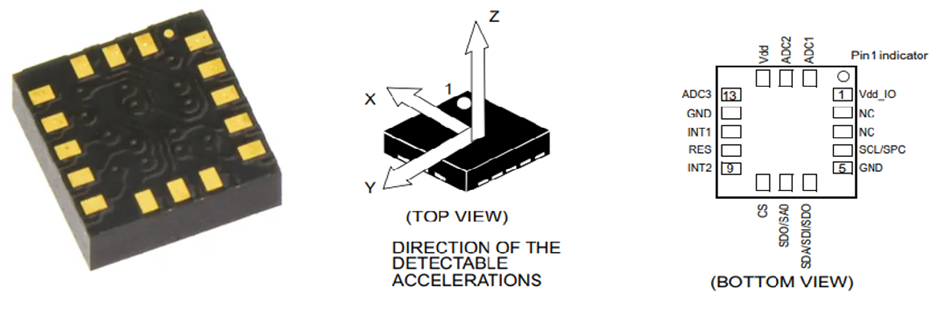
\includegraphics[width=0.8\textwidth]{images/lis.png}
		\caption{Cảm biến gia tốc LIS3DH và sơ đồ chân kết nối}
		\label{lis}
\end{figure}

LIS3DH với thang đo đầy đủ khá rộng cho phép người phát triển có thể lựa chọn các giá trị ± 2g / ± 4g / ± 8g / ± 16g và có khả năng đo gia tốc với tần số ở lối ra từ 1 Hz đến 5.3 kHz. Thiết bị có thể được cấu hình để tạo ra tín hiệu ngắt bằng cách sử dụng hai sự kiện đánh thức / rơi tự do theo quán tính độc lập cũng như theo vị trí của chính thiết bị. Người dùng cuối có thể lập trình ngưỡng và thời gian của bộ tạo ngắt. LIS3DH tích hợp bộ đệm 32 cấp vào ra tuần tự (FIFO) cho phép người dùng lưu trữ dữ liệu nhằm hạn chế sự can thiệp của bộ xử lý chủ. LIS3DH được đảm bảo hoạt động trong phạm vi nhiệt độ mở rộng từ -40°C đến +85°C. LIS3DH có kích thước nhỏ gọn, thích hợp trong thiết kế mạch đo nhỏ gọn, Hình~\ref{lis}. Thiết bị hỗ trợ dải điện áp cung cấp rộng, dao động từ 1.71 V đến 3.6 V, cho phép linh hoạt trong thiết kế nguồn. Ngoài ra, cảm biến còn tích hợp nguồn cung cấp I/O độc lập ở mức 1.8 V, đồng thời vẫn đảm bảo khả năng tương thích với các hệ thống điện áp khác nhau. Một trong những ưu điểm nổi bật của LIS3DH là chế độ tiêu thụ dòng điện cực thấp, chỉ khoảng 2~$\mu$A trong chế độ tiết kiệm năng lượng, điều này rất quan trọng đối với các hệ thống hoạt động liên tục trong thời gian dài. Thiết bị sử dụng giao diện kỹ thuật số I2C/SPI cho đầu ra dữ liệu, giúp đơn giản hóa việc truyền nhận thông tin giữa cảm biến và bộ xử lý trung tâm. Cảm biến cung cấp đầu ra dữ liệu với độ phân giải 10 bit, cho phép ghi nhận chính xác các thay đổi nhỏ trong chuyển động. Bên cạnh đó, LIS3DH còn được trang bị hai bộ ngắt lập trình độc lập, hỗ trợ phát hiện các chuyển động đặc biệt như rơi tự do và chuyển động nhanh, đồng thời tích hợp tính năng phát hiện định hướng không gian 4D/6D, rất hữu ích trong việc phân loại tư thế ngủ. Thiết bị này đáp ứng các tiêu chuẩn môi trường nghiêm ngặt như ECOPACK®, RoHS và "Green", bảo đảm thân thiện với môi trường và an toàn cho người sử dụng. Trong ngữ cảnh theo dõi tư thế ngủ, khi người đang ngủ thay đổi vị trí, gia tốc cơ thể thường dao động trong phạm vi ±2g. Với độ phân giải đầu ra 10 bit, tức 1024 mức chia, hệ thống có thể đạt độ phân giải lý thuyết khoảng 0.004g. Độ phân giải này là hoàn toàn phù hợp để ghi nhận các thay đổi chậm và nhỏ đặc trưng trong quá trình chuyển đổi tư thế khi ngủ, từ đó hỗ trợ hiệu quả cho các mô hình phân tích bằng trí tuệ nhân tạo.


\section{Nghiên cứu, lựa chọn vi xử lý}

Với sự phát triển vượt bậc và đa dạng của công nghệ chế tạo, có rất nhiều cấu hình phần cứng được nhiều nhóm tác giả lựa chọn phù hợp với các mục đích khác nhau. Trong đó, \cite{p_1} các tác giả đã sử dụng máy tính đơn Raspberry Pi kết hợp các điện trở cảm biến lực để phát hiện 4 tư thế ngủ với sự lấy nhãn từ video theo dõi người bệnh trong suốt quá trình lấy mẫu. Kwasnicki và cộng sự đã phát triển hệ thống ngủ có thể đeo (wearable sleep system) sử dụng bộ xử lý công suất thấp TI MSP430 và mô-đun RF Chipcon CC2420 cho truyền thông không dây kết hợp với cảm biến gia tốc 3 trục ADXL330, con quay hồi chuyển InvenSense ITG-3200, Honeywell HMC5843 để đo từ trường xác định 99.5\% chính xác 4 tư thế ngủ \cite{p_2}. Tuy nhiên, các thiết bị vẫn yêu cầu một nguồn nặng lượng khiến cho tính liên tục bị hạn chế đáng kể. I.Yun và cộng sự đã phát triển thiết bị theo dõi tư thế ngủ của trẻ nhỏ sử dụng vi xử lý ATmega328P-PU cùng module Bluetooth kết hợp cảm biến gia tốc ADXL335 được đặt trên bụng đã nhưng lựa chọn về mặt cấu hình thiết bị và chế tạo ra mạch cung cấp năng lượng cho những thành phần cần thiết \cite{p_3}. Từ đó, giảm thiếu đáng kể mức tiêu thụ năng lượng và vẫn giữ nguyên độ chính xác nhưng khá bất tiện cho trẻ nhỏ.

\begin{figure}[!ht]
		\centering
 		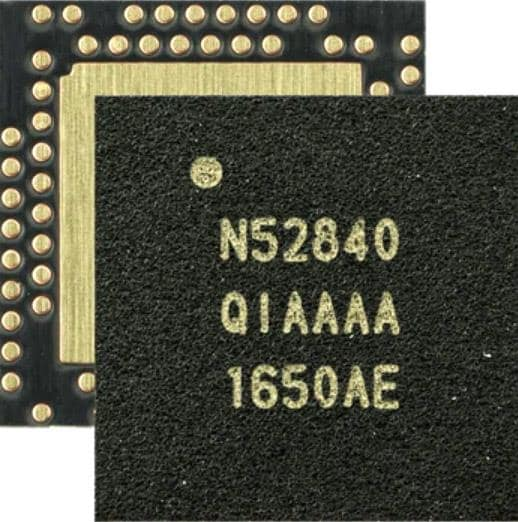
\includegraphics[width=0.8\textwidth]{images/NRF52840-QFA_SPL.jpg}
		\caption{Nordic Semiconductor NRF52840}
		\label{lis}
\end{figure}

Sau quá trình khảo sát, đánh giá và so sánh giữa các lựa chọn vi xử lý phổ biến hiện nay, tác giả quyết định lựa chọn vi xử lý nRF52840 \cite{nrf} cho hệ thống được đề xuất, dựa trên những ưu điểm nổi bật như kích thước nhỏ gọn, mức tiêu thụ năng lượng thấp và khả năng tích hợp Bluetooth năng lượng thấp (Bluetooth Low Energy – BLE). nRF52840 là vi xử lý cao cấp nhất trong dòng họ nRF52 do hãng Nordic Semiconductor phát triển. Đây là một hệ thống tích hợp trên một vi mạch (System-on-Chip – SoC), được thiết kế tối ưu cho các ứng dụng yêu cầu mức tiêu thụ năng lượng cực thấp, đặc biệt là trong các mạng không dây tầm ngắn. Vi xử lý này tích hợp bộ thu phát đa giao thức hoạt động ở băng tần 2.4 GHz, sử dụng kiến trúc CPU Arm Cortex-M4F với tốc độ xung nhịp 64 MHz, cùng bộ xử lý dấu phẩy động (FPU) và dung lượng bộ nhớ gồm 1 MB bộ nhớ Flash và 256 KB RAM. Bên cạnh đó, nRF52840 hỗ trợ chuẩn Bluetooth 5.3 với khả năng giao tiếp đa giao thức, cho phép tăng cường phạm vi truyền dữ liệu, cải thiện tốc độ truyền và giảm tiêu thụ năng lượng. Bộ tính năng bảo mật được tích hợp một cách đầy đủ, đáp ứng các yêu cầu ngày càng cao trong bảo vệ dữ liệu và truyền thông không dây. Vi xử lý này còn sở hữu khả năng quản lý năng lượng linh hoạt, có thể hoạt động trong dải điện áp rộng từ +5.5V xuống đến +1.7V, cho phép thiết bị hoạt động trực tiếp từ nguồn pin hoặc cổng USB. Về khả năng giao tiếp ngoại vi, nRF52840 cung cấp cấu hình đa dạng, bao gồm tối đa hai giao tiếp I2C, bốn giao tiếp SPI ở chế độ master và ba SPI ở chế độ slave, cùng bốn kênh PWM tích hợp EasyDMA. Ngoài ra, thiết bị còn hỗ trợ năm bộ định thời 32-bit, phù hợp với các ứng dụng đòi hỏi độ chính xác cao trong xử lý thời gian thực.



\subsection{Vi điều khiển ARM Cortex-M4}

Kiến trúc ARM có nhiều dòng vi xử lý khác nhau, được phát triển và nâng cấp liên tục nhằm đáp ứng nhu cầu đa dạng trong lĩnh vực công nghệ nhúng. Trong đó, dòng Cortex-M thuộc kiến trúc ARMv7 đã trở thành nền tảng phổ biến cho các hệ thống nhúng sử dụng vi điều khiển nhờ vào hiệu suất cao, khả năng mở rộng và mức tiêu thụ năng lượng tối ưu. Dòng Cortex-M bao gồm nhiều phiên bản như Cortex-M0, Cortex-M0+, Cortex-M1, Cortex-M3, Cortex-M4 và Cortex-M7, mỗi phiên bản được thiết kế để phục vụ cho các mức độ yêu cầu hiệu năng khác nhau \cite{arm_cortex_m_comparison}. Các vi xử lý thuộc họ Cortex-M chủ yếu được ứng dụng trong các hệ thống nhúng thời gian thực, nơi yêu cầu sự cân bằng giữa hiệu suất xử lý, tiêu thụ năng lượng và chi phí. Một số vi xử lý ARM khác, không thuộc họ Cortex-M, được sử dụng trong các thiết bị hiệu suất cao như điện thoại thông minh và máy tính bảng, vốn yêu cầu cấu hình phần cứng mạnh hơn và khả năng xử lý đa tác vụ cao hơn. Ngoài ra, hiện nay ứng dụng trí tuệ nhân tạo (AI) tại thiết bị biên (Edge AI) đang ngày càng phổ biến, đặc biệt trong các lĩnh vực như nhà thông minh, thiết bị đeo, giám sát an ninh và công nghiệp 4.0. Với khả năng xử lý tín hiệu số (DSP) và hỗ trợ các mạng nơ-ron nhỏ gọn, các vi xử lý Cortex-M, đặc biệt là dòng Cortex-M4, đang được khai thác để triển khai các mô hình học sâu nhẹ (tinyML) ngay trên vi điều khiển \cite{electronics11162545}\cite{applicationCortexM4}.

Nhờ vào đặc điểm kỹ thuật như vậy, Cortex-M4 được ứng dụng rộng rãi trong nhiều lĩnh vực khác nhau, bao gồm điều khiển động cơ, công nghiệp ô tô, hệ thống quản lý năng lượng, âm thanh nhúng và các hệ thống tự động hóa công nghiệp. Tính linh hoạt và hiệu quả về hiệu suất – năng lượng giúp Cortex-M4 trở thành một trong những vi xử lý được ưa chuộng nhất trong phát triển hệ thống nhúng hiện đại.

Theo tài liệu \cite{cortexM4}, bộ vi xử lý Cortex-M4 là một vi xử lý 32-bit sử dụng kiến trúc tập lệnh giảm (RISC), được thiết kế theo kiến trúc Harvard, trong đó bus dữ liệu và bus lệnh được tách biệt nhằm tối ưu tốc độ truyền tải và xử lý. Vi xử lý này hỗ trợ đầy đủ tập lệnh Thumb-1 (16-bit) cũng như Thumb-2 (kết hợp 16-bit và 32-bit), mang lại sự linh hoạt trong việc mã hóa lệnh và hiệu quả bộ nhớ. Về mặt hiệu năng, Cortex-M4 đạt được từ 1,25 đến 1,95 DMIPS trên mỗi MHz (Dhrystone Million Instructions Per Second per MHz), cho thấy khả năng xử lý tốt trong các ứng dụng nhúng yêu cầu độ chính xác cao. Bộ xử lý hỗ trợ lên đến 240 tín hiệu ngắt, bao gồm các ngắt ngoại lệ không chắn được (Non-Maskable Interrupts – NMI), cùng với khả năng cấu hình từ 8 đến 256 mức ngắt ưu tiên khác nhau. Điều này giúp hệ thống xử lý hiệu quả các tác vụ thời gian thực, đặc biệt trong môi trường nhúng có nhiều ngắt cạnh tranh xảy ra đồng thời.


\begin{figure}[!ht]
		\centering
 		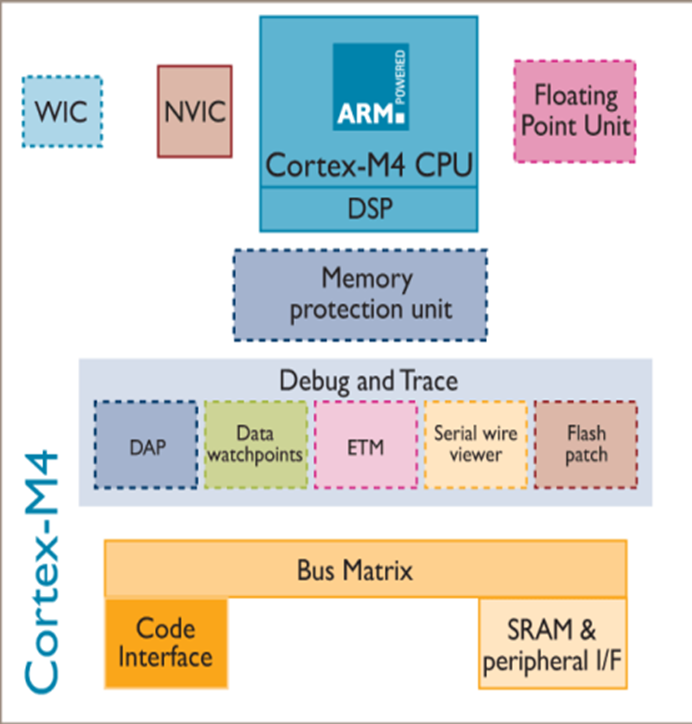
\includegraphics[width=0.8\textwidth]{images/cortexM4.png}
		\caption{Thành phần chính của vi điều khiển Cortex-M4}
		\label{cortexM4}
\end{figure}

Kết nối bus được mô tả trong Hình~\ref{cortexM4} cho phép truyền dữ liệu đồng thời trên nhiều bus khác nhau, đồng thời cung cấp khả năng quản lý truyền dữ liệu hiệu quả, chẳng hạn như sử dụng bộ đệm ghi và điều khiển hướng bit hoạt động (bit-banding). Hệ thống cũng có thể bao gồm các cầu bus (bus bridges) nhằm kết nối nhiều loại bus vào một mạng duy nhất sử dụng chung không gian bộ nhớ. Ngoài ra, bộ xử lý được trang bị hệ thống hỗ trợ gỡ lỗi tích hợp, bao gồm khả năng kiểm soát gỡ lỗi, thiết lập điểm ngắt (breakpoint) chương trình và điểm theo dõi dữ liệu (watchpoint). Khi xảy ra sự kiện gỡ lỗi, hệ thống có thể tạm dừng trạng thái hoạt động của lõi xử lý để phục vụ việc phân tích và xử lý lỗi.

Bên cạnh đó, kiến trúc Cortex-M4 tích hợp Bộ điều khiển ngắt vectored lồng nhau (Nested Vectored Interrupt Controller – NVIC) với khả năng hỗ trợ lên đến 240 tín hiệu yêu cầu ngắt, bao gồm cả ngắt không chắn được (NMI). NVIC hỗ trợ xử lý ngắt lồng nhau một cách tự động bằng cách so sánh mức ưu tiên giữa các yêu cầu ngắt với mức ưu tiên hiện tại đang được xử lý.

Đối với các ứng dụng yêu cầu tiết kiệm năng lượng, hệ thống còn được trang bị bộ đánh thức ngắt (Wake-up Interrupt Controller – WIC), cho phép đưa bộ vi điều khiển vào chế độ nghỉ bằng cách tắt hầu hết các thành phần không cần thiết, đồng thời duy trì khả năng đánh thức hệ thống khi phát hiện một yêu cầu ngắt. Ngoài ra, cơ chế bảo vệ bộ nhớ cũng được tích hợp nhằm đảm bảo an toàn cho hệ thống, ví dụ như chỉ cho phép truy cập đọc tại một số vùng bộ nhớ hoặc ngăn người dùng truy cập vào các vùng dữ liệu đặc quyền của hệ điều hành hoặc ứng dụng hệ thống.


\subsection{Bluetooth năng lượng thấp}
    
\begin{figure}[!ht]
		\centering
 		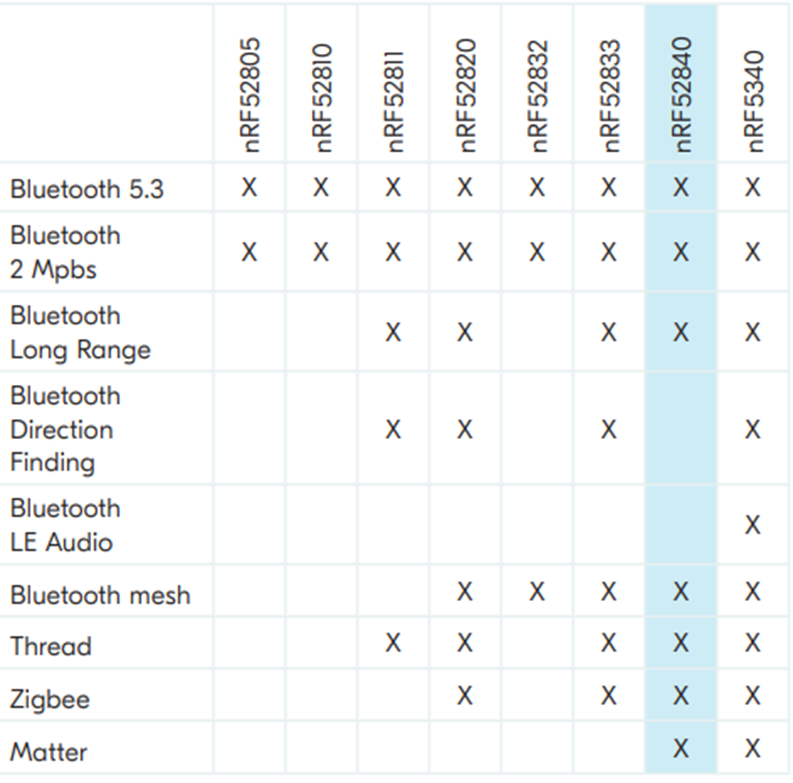
\includegraphics[width=0.8\textwidth]{images/ble.png}
		\caption{Các kiểu kết nối không dây trong họ chip nRF52}
		\label{ble}
\end{figure}

Bluetooth năng lượng thấp (Bluetooth Low Energy – BLE) là một chuẩn kết nối không dây chi phí thấp, được thiết kế tối ưu cho các ứng dụng tiêu thụ điện năng thấp, đặc biệt phù hợp với các thiết bị hoạt động bằng pin kích thước nhỏ. BLE hoạt động trong băng tần ISM 2.4 GHz, hỗ trợ thông lượng ứng dụng lên đến 1.4 Mbps, cho phép truyền dữ liệu hiệu quả trong khi vẫn duy trì mức tiêu thụ năng lượng tối thiểu.

Về mặt bảo mật, BLE tích hợp các cơ chế mã hóa và xác thực nhằm đảm bảo tính bí mật, toàn vẹn và riêng tư của dữ liệu truyền qua mạng. Công nghệ này đã trở thành một phần tiêu chuẩn trong hầu hết các thiết bị di động hiện đại như smartphone, máy tính bảng, và laptop, đồng thời được hỗ trợ đầy đủ trên các hệ điều hành phổ biến bao gồm iOS, Android, macOS, Windows 10 và Linux. Bluetooth 5 là bước phát triển đột phá tiếp theo kể từ khi BLE được giới thiệu trong chuẩn Bluetooth 4.0, mang đến hàng loạt cải tiến đáng kể giúp mở rộng phạm vi ứng dụng và nâng cao hiệu suất hệ thống. Một trong những cải tiến nổi bật là chế độ 2 Mbps, cho phép tăng gấp đôi tốc độ truyền lý thuyết, tương ứng với thông lượng thực tế lên đến 1.4 Mbps. Quan trọng hơn, chế độ này còn giúp giảm đáng kể mức tiêu thụ năng lượng – cụ thể là giảm một nửa năng lượng tiêu thụ trên mỗi bit dữ liệu – từ đó kéo dài thời gian hoạt động của thiết bị hoặc cho phép sử dụng các nguồn năng lượng nhỏ và chi phí thấp hơn \cite{BLE}. 

Bên cạnh đó, tính năng Advertising Extensions (mở rộng quảng cáo) đã cách mạng hóa cơ chế phát sóng của BLE. Các gói quảng cáo giờ đây có thể chứa lượng dữ liệu gấp 8 lần so với phiên bản trước, cho phép truyền tải các khối dữ liệu lớn hơn mà không cần thiết lập kết nối ngay lập tức. Đồng thời, các gói quảng cáo có thể được xâu chuỗi để tạo thành các tập tin quảng cáo phức hợp. Tính năng lựa chọn kênh được tối ưu hóa giúp tăng cường độ ổn định và khả năng chống nhiễu trong các môi trường có mật độ thiết bị cao. Đặc biệt, chế độ Long Range mở rộng đáng kể phạm vi truyền thông của BLE, cho phép các thiết bị duy trì kết nối trong toàn bộ không gian của một ngôi nhà thông minh hoặc trong các ứng dụng IoT công nghiệp quy mô vừa và nhỏ.




\begin{figure}[!ht]
	\centering
 	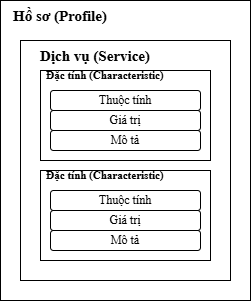
\includegraphics[width=0.5\textwidth]{images/gatt.drawio.png}
	\caption{Cấu trúc của GATT}
	\label{gatt}
\end{figure}

Ngoài các tính năng nổi bật đã đề cập, vi xử lý nRF52840 còn hỗ trợ Bluetooth Mesh, một công nghệ mạng lưới tiên tiến được phát triển nhằm mở rộng đáng kể khả năng truyền thông của Bluetooth Low Energy (BLE). Bluetooth Mesh cho phép thiết lập mạng truyền thông nhiều-đến-nhiều (many-to-many), hoạt động ổn định trong các hệ thống có thể lên đến hàng nghìn nút mạng, phù hợp với các ứng dụng IoT quy mô lớn như nhà thông minh, chiếu sáng công nghiệp, giám sát môi trường và hệ thống cảm biến phân tán.

Bluetooth Mesh sử dụng BLE làm lớp truyền tải vật lý, trong đó các thông điệp được đóng gói trong các gói quảng cáo (advertising packets) hoặc gói GATT – còn được gọi là gói cấu hình thuộc tính chung (Generic Attribute Profile – GATT). Khi một thiết bị di động hoặc máy chủ trung tâm kết nối với một nút BLE bất kỳ trong mạng Mesh, nút này có thể chuyển tiếp (relay) thông điệp đến các nút khác trong mạng theo một kiến trúc định tuyến phân tán, như minh họa trong Hình~\ref{ble}.

Cấu trúc logic của BLE được tổ chức dựa trên mô hình GATT. GATT định nghĩa cách hai thiết bị BLE truyền dữ liệu qua lại bằng các thành phần logic gọi là dịch vụ (services) và đặc tính (characteristics). Giao tiếp GATT dựa trên Attribute Protocol (ATT) – một giao thức định hướng dữ liệu, nơi các dịch vụ và đặc tính được lưu trữ và nhận dạng bằng các mã định danh (UUID) có độ dài 16-bit hoặc 128-bit. Hình~\ref{gatt} minh họa cấu trúc phân cấp của GATT, trong đó một thiết bị ngoại vi BLE cung cấp nhiều dịch vụ, mỗi dịch vụ lại bao gồm một hoặc nhiều đặc tính có thể được đọc, ghi hoặc thông báo (notify) tùy theo cấu hình.

Điều đặc biệt quan trọng trong giao tiếp GATT là tính chất kết nối độc quyền (exclusive connection): tại một thời điểm nhất định, một thiết bị ngoại vi chỉ có thể kết nối với một thiết bị trung tâm duy nhất. Ngay khi kết nối được thiết lập, thiết bị ngoại vi sẽ ngừng quảng cáo, khiến các thiết bị khác không thể phát hiện hoặc kết nối với nó cho đến khi kết nối hiện tại bị ngắt.

Hồ sơ (Profile) là tập hợp các dịch vụ được xác định trước, được tiêu chuẩn hóa bởi tổ chức Bluetooth SIG hoặc do nhà phát triển thiết kế tùy chỉnh. Mỗi dịch vụ đại diện cho một thực thể logic trong hệ thống BLE, chứa một hoặc nhiều đặc tính, là đơn vị dữ liệu cơ bản nhất. Một đặc tính bao gồm giá trị chính (value), mô tả (description), và các thuộc tính điều khiển quyền truy cập như chỉ đọc, chỉ ghi hoặc hỗ trợ thông báo.

Chẳng hạn, một ứng dụng BLE có thể triển khai Dịch vụ UART tùy chỉnh, bao gồm hai đặc tính đại diện cho kênh truyền (TX) và kênh nhận (RX), trong đó một đặc tính chỉ cho phép đọc và đặc tính còn lại cho phép ghi từ phía thiết bị trung tâm.

Với các khả năng kỹ thuật tiên tiến như trên – bao gồm hỗ trợ Bluetooth Mesh, giao tiếp GATT hiệu quả, khả năng quản lý năng lượng linh hoạt, bảo mật tích hợp và khả năng xử lý tín hiệu số – nRF52840 được xem là lựa chọn phù hợp và chiến lược trong khuôn khổ triển khai hệ thống được đề xuất trong luận văn này.


\subsection{Thiết bị thử nghiệm}
Trong khuôn khổ của khoá luận, vì lý do thời gian và sự an toàn nên tác giả sử dụng bộ kit Adafruid PlayGround để thực nghiệm. Trong bộ kit có 1 cảm biến gia tốc MEMS LIS3DH ở chính giữa. Cảm biến gia tốc này thường dùng trong điện thoại và các thiết bị điện tử khác có thể cảm nhận độ nghiêng, trọng lực, chuyển động và các hiệu ứng 'chạm'. Thông tin mà tác giả có được, chi phí cho mỗi một kit từ Adafruit khoảng 25 USD \cite{ada_price}. LIS3DH được kết nối với các chân SPI phần cứng và có chân chọn chip (CS) trên chân số 8 và đầu ra ngắt tùy chọn trên chân số 7 (còn được gọi là IRQ \# 4). Có thể phát hiện các giá trị gia tốc theo 3 trục X, Y và Z. Giá trị dương là mặt màu của kit. Trục X là hướng tới giắc cắm USB. Trục Y trục hướng sang bên trái. Đối với Z là hướng thẳng hướng lên.

\textbf{Các thành phần trên bộ kit Adafruit Circuit PlayGround\cite{ada_overview}:}

\begin{figure}[!ht]
		\centering
 		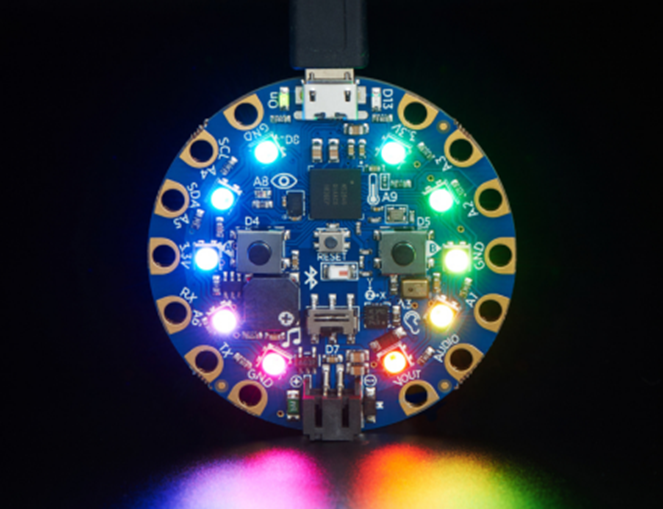
\includegraphics[width=0.8\textwidth]{images/ada.png}
		\caption{Hình ảnh kit Adafruit PlayGround}
		\label{ada}
\end{figure}

\begin{figure}[!ht]
		\centering
 		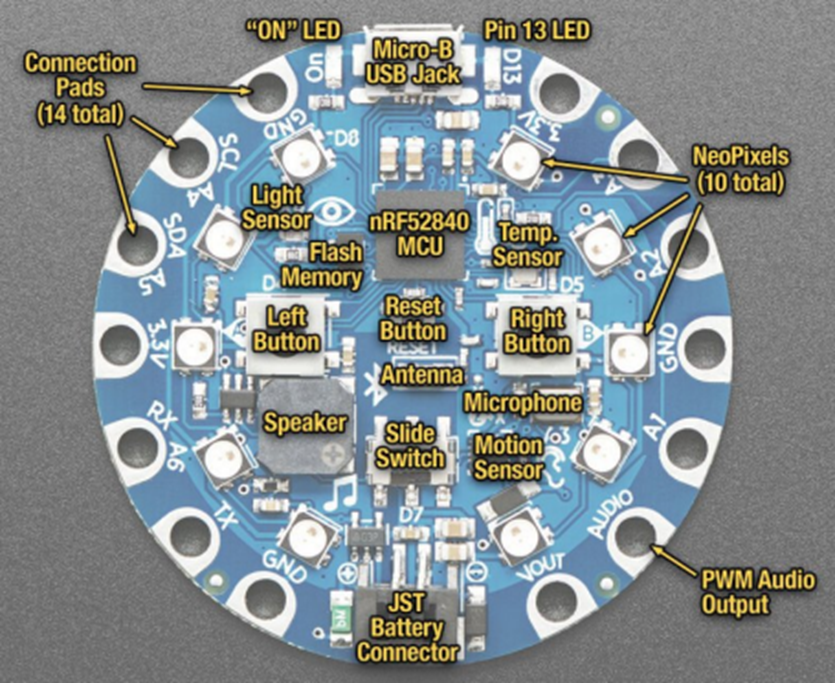
\includegraphics[width=0.8\textwidth]{images/detail_ada.png}
		\caption{Cấu trúc các thành phần trên Circuit PlayGround}
		\label{detail_ada}
\end{figure}

\begin{itemize}
    \item 1 x bộ xử lý nRF52840 Cortex M4 với hỗ trợ Bluetooth Low Energy
    \item 10 x NeoPixels mini, mỗi cái có thể hiển thị bất kỳ màu nào
    \item 1 x Cảm biến chuyển động (gia tốc kế ba trục LIS3DH với phát hiện chạm, phát hiện rơi tự do)
    \item 1 x Cảm biến nhiệt độ (nhiệt điện trở)
    \item 1 x Cảm biến ánh sáng (phototransistor). Cũng có thể hoạt động như một cảm biến màu và cảm biến xung
    \item 1 x Cảm biến âm thanh (micrô MEMS)
    \item 1 x Loa mini với bộ khuếch đại lớp D (loa từ tính 7,5mm / còi)
    \item 2 x Nút ấn, có nhãn A và B
    \item 1 x Công tắc trượt
    \item 8 x chân đầu vào / đầu ra thân thiện với alligator-clip
    \item Bao gồm I2C, UART, 6 chân có thể làm đầu vào tương tự, nhiều đầu ra PWM
    \item Đèn LED "On" màu xanh lục để bạn biết nó được cấp nguồn
    \item 2 MB dung lượng lưu trữ SPI Flash, được sử dụng chủ yếu với CircuitPython để lưu trữ mã và thư viện.
    \item Cổng MicroUSB để lập trình và gỡ lỗi
    \item Cổng USB có thể hoạt động như cổng nối tiếp, bàn phím, chuột, cần điều khiển hoặc MIDI!
    \item Thiết kế ăng-ten đã được tối ưu và có thêm một chốt cho phép người dùng tắt nguồn của NeoPixels, micrô và cảm biến nhiệt độ / ánh sáng để chỉ có gia tốc kế hoạt động, để sử dụng năng lượng thấp!
    \item Đường kính ngoài: ~ 50.6 mm / ~ 2,0 "
    
    
\end{itemize}






\begin{figure}[!]
		\centering
 		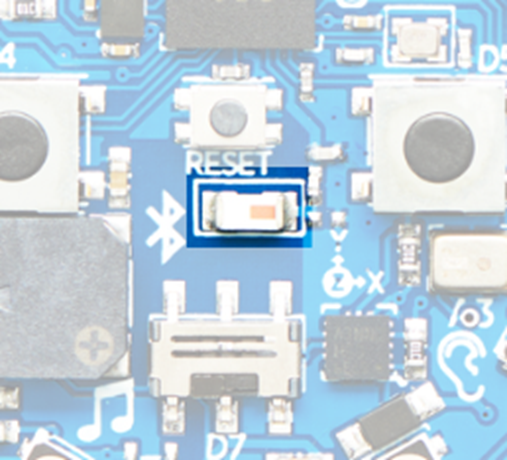
\includegraphics[width=0.8\textwidth]{images/angten.png}
		\caption{Vị trí của ăng ten trên bo mạch}
		\label{angten}
\end{figure}

\begin{figure}[!]
		\centering
 		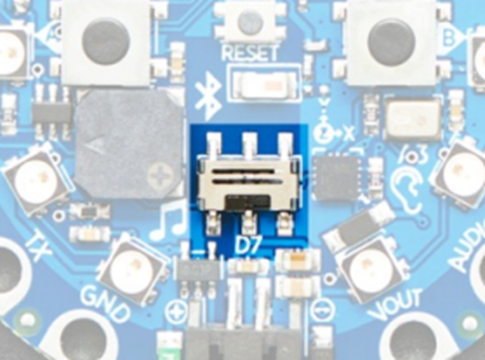
\includegraphics[width=0.8\textwidth]{images/switch.png}
		\caption{Vị trí của chân chuyển đổi cấu hình trên bo mạch}
		\label{switch}
\end{figure}

\textbf{Năng lượng và dữ liệu:}
\begin{itemize}
    \item Đầu nối USB Micro B ở trên cùng của bo mạch cho phép giao tiếp nguồn hoặc USB (bộ nạp khởi động tiếp, HID, v.v.). 
    \item Chân cấp nguồn ngoài có thể sử dụng đầu vào DC 6V và có các bảo vệ chống phân cực ngược, quá dòng và nhiệt. Mạch bên trong sẽ sử dụng nguồn điện đầu vào của pin hoặc nguồn điện USB, chuyển từ nguồn này sang nguồn khác một cách an toàn. Nếu cả hai được kết nối, nó sẽ sử dụng cái nào có điện áp cao hơn. Hoạt động hiệu quả với pin Lithium Polymer hoặc các gói pin 3xAAA của tác giả với đầu nối JST ở cuối. Không có sạc pin tích hợp.
\end{itemize}


\textbf{Ăng ten cho BLE}

Ăng-ten Bluetooth nằm ở giữa bo mạch như trên Hình~\ref{angten}. Cần phải đảm bảo không có linh kiện nào gần ăng-ten có thể gây nhiễu, hoặc bề mặt kim loại để tối ưu tầm hoạt động của ăng-ten.




\textbf{Chân chuyển đổi cấu hình}
Công tắc trượt gần phía dưới trung tâm của Circuit Playground Bluefruit. nó được kết nối với D7 kỹ thuật số, Hình~\ref{switch}. Công tác sử dụng điện trở kéo để thiết lập cấu hình tiêu thụ năng lượng cao hoặc cấu hình tiêu thụ năng lượng thấp. 







\section{Kỹ thuật thu thập và xử lý tín hiệu}
\subsection{Lập trình vi xử lý}

\begin{figure}[!]
		\centering
 		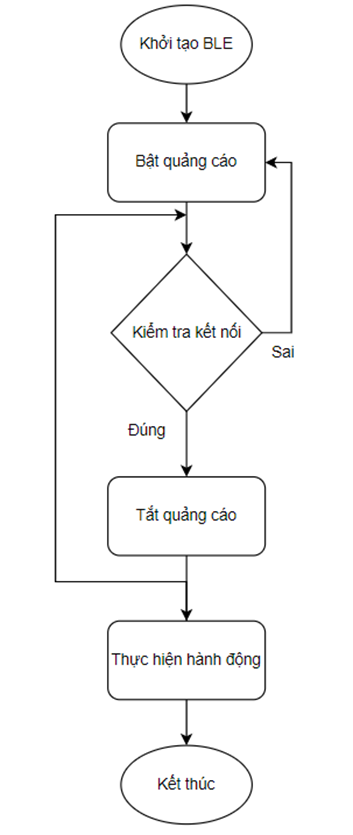
\includegraphics[width=0.5\textwidth]{images/flowBLE.png}
		\caption{Lưu đồ hoạt động của thiết bị BLE}
		\label{flowBLE}
\end{figure}

\begin{lstlisting}[float,language=C,caption=Tập lệnh khởi tạo và kết nối Bluetooth từ thư viện của AdaFruit, label=arduinoBLE,captionpos=b]
void startAdv(void)
{
  // Advertising packet
  Bluefruit.Advertising.addFlags(BLE_GAP_ADV_FLAGS_LE_ONLY_GENERAL_DISC_MODE);
  Bluefruit.Advertising.addTxPower();

  // Include HRM Service UUID
  Bluefruit.Advertising.addService(positionService);

  // Include Name
  Bluefruit.Advertising.addName();
  
  /* Start Advertising
   * - Enable auto advertising if disconnected
   * - Interval:  fast mode = 20 ms, slow mode = 152.5 ms
   * - Timeout for fast mode is 30 seconds
   * - Start(timeout) with timeout = 0 will advertise forever (until connected)
   * 
   * For recommended advertising interval
   * https://developer.apple.com/library/content/qa/qa1931/_index.html   
   */
  Bluefruit.Advertising.restartOnDisconnect(true);
  Bluefruit.Advertising.setInterval(32, 244);    // in unit of 0.625 ms
  Bluefruit.Advertising.setFastTimeout(30);      // number of seconds in fast mode
  Bluefruit.Advertising.start(0);                // 0 = Don't stop advertising after n seconds  
}
\end{lstlisting}



Tác giả thực hiện lập trình trên Arduino IDE và thư viện Circuit Playground. Trong phần khởi tạo (setup) các bản tin quảng cáo (advertising) sẽ được khởi tạo và được thực thi. Tiếp theo là cấu hình các hàm kết nối, ngắt kết nối, cấu hình chung \gls{GATT} Hình~\ref{flowBLE}.



Trong mã nguồn \ref{arduinoBLE}, hàm startAdv có nhiệm vụ khởi tạo tên, thêm các dịch vụ và bắt đầu quảng cáo cho thiết bị. Sau đó, cấu hình cho \gls{BLE} theo định dạng \gls{GATT} sẽ được thiết lập. Đầu tiên, khởi tạo dịch vụ $positionService$ có mã định dang duy nhất(Universally Unique IDentifier - UUID) là 0x1821. Tiếp theo, thêm các đặc tính $BLE-GATT-UNIT-ACCELERATION
-METRES-PER-SECOND-SQUARED
$ và $BLE-GATT-UNIT-ANGULAR-ACCELERATION
-RADIAN-PER-SECOND-SQUARED
$ có UUID lần lượt là 0x2713 và 0x2744. Hàm cấu hình setupPosition được tác giả sử dụng để cấu hình chi tiết GATT cho BLE. Có 2 service được khởi tạo là gia tốc và con quay hồi chuyển. Tuy nhiên, trong khuôn khổ khóa luận tác giả tập trung vào giá trị gia tốc của cảm biến gia tốc. 


\begin{lstlisting}[float,language=C,caption=Tập lệnh khởi tạo các thuộc tính GATT, label=gattBle,captionpos=b]
void setupPosition(void)
{
 
  positionService.begin();

  accelerometerCharacter.setProperties(CHR_PROPS_NOTIFY+CHR_PROPS_READ+CHR_PROPS_WRITE );
  accelerometerCharacter.setPermission(SECMODE_OPEN, SECMODE_NO_ACCESS);
  accelerometerCharacter.setFixedLen(9);
  accelerometerCharacter.setCccdWriteCallback(cccd_callback);  // Optionally capture CCCD updates
  accelerometerCharacter.begin();
  uint8_t accelerometerData[9] = { 0b00000000, 0b00000000, 0b00000000,0b00000000,0b00000000,0b00000000,0b00000000,0b00000000,0b00000000}; // Set the characteristic to use 8-bit values, with the sensor connected and detected
  accelerometerCharacter.write(accelerometerData, 9);

  gyroscopeCharacter.setProperties(CHR_PROPS_READ);
  gyroscopeCharacter.setPermission(SECMODE_OPEN, SECMODE_NO_ACCESS);
  gyroscopeCharacter.setFixedLen(1);
  gyroscopeCharacter.begin();
  gyroscopeCharacter.write8(2);    // Set the characteristic to 'Wrist' (2)
}

\end{lstlisting}


\begin{lstlisting}[float,language=C,caption=Gửi dữ liệu từ BLE, label=sendBle,captionpos=b]
void setupPosition(void)
{
 
  positionService.begin();

  accelerometerCharacter.setProperties(CHR_PROPS_NOTIFY+CHR_PROPS_READ+CHR_PROPS_WRITE );
  accelerometerCharacter.setPermission(SECMODE_OPEN, SECMODE_NO_ACCESS);
  accelerometerCharacter.setFixedLen(9);
  accelerometerCharacter.setCccdWriteCallback(cccd_callback);  // Optionally capture CCCD updates
  accelerometerCharacter.begin();
  uint8_t accelerometerData[9] = { 0b00000000, 0b00000000, 0b00000000,0b00000000,0b00000000,0b00000000,0b00000000,0b00000000,0b00000000}; // Set the characteristic to use 8-bit values, with the sensor connected and detected
  accelerometerCharacter.write(accelerometerData, 9);

  gyroscopeCharacter.setProperties(CHR_PROPS_READ);
  gyroscopeCharacter.setPermission(SECMODE_OPEN, SECMODE_NO_ACCESS);
  gyroscopeCharacter.setFixedLen(1);
  gyroscopeCharacter.begin();
  gyroscopeCharacter.write8(2);    // Set the characteristic to 'Wrist' (2)
}

\end{lstlisting}


\textbf{setProperties} - phương thức để thay đổi thuộc tính liên quan đến quyền BLE có thể được đặt thành một hoặc nhiều lựa chọn sau:

\begin{itemize}
    \item CHR\_PROPS\_BROADCAST = bit (0)
    
    \item CHR\_PROPS\_READ = bit (1)
    
    \item CHR\_PROPS\_WRITE\_WO\_RESP = bit (2)
    
    \item CHR\_PROPS\_WRITE = bit (3)
    
    \item CHR\_PROPS\_NOTIFY = bit (4)
    
    \item CHR\_PROPS\_INDICATE = bit (5)
\end{itemize}
Ngoài ta còn nhiều hàm như \textbf{setPermission} để cài đặt tính bảo mật. \textbf{setFixedLen} để cấu hình gửi bao nhiêu bit.





\begin{figure}[!]
		\centering
 		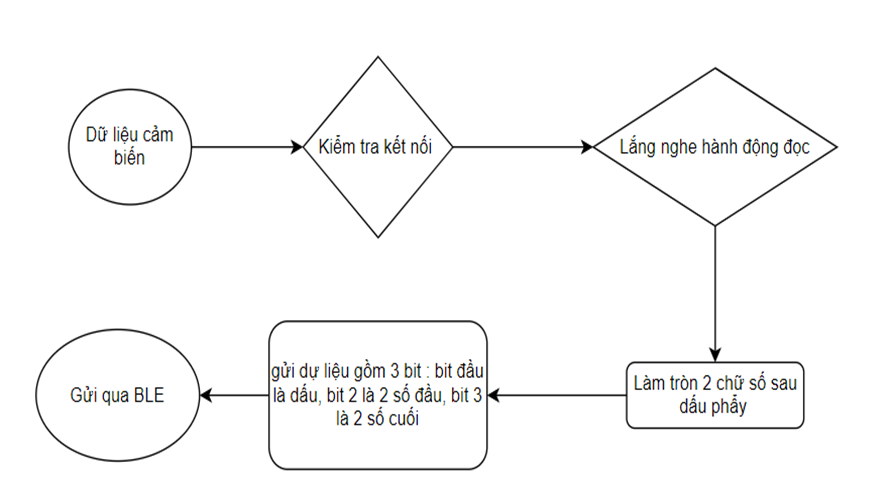
\includegraphics[width=1\textwidth]{images/sendBleFlow.png}
		\caption{Lưu đồ luồng gửi thông tin BLE}
		\label{sendBleFlow}
\end{figure}


















\subsection{Hiệu chuẩn cảm biến}
Việc thu nhận dữ liệu và tiền xử lý dữ liệu là cần thiết trong các hệ đo. Cảm biến mặc dù đã được hiệu chuẩn tại nơi sản xuất nhưng vẫn cần được hiệu chuẩn trong hệ thống và môi trường đo thực tế. Mục đích của việc hiệu chuẩn là cải thiện hiệu năng của cảm biến bằng cách loại bỏ hoặc giảm thiểu sai số trong dữ liệu đầu ra cảm biến. Lỗi cảm biến phân làm 2 loại i) lỗi mặc định và ii) lỗi ngẫu nhiên. Để xử lý lỗi mặc định, tác giả tác giả sử dụng gia tốc trọng trường để hiệu chuẩn cảm biến. Giá trị một trục gia tốc của cảm biến xoay lên trên so với mặt phẳng ngang sẽ nhận giá trị là -1g, khi xoay xuống dưới nhận giá trị là +1g. Hiệu chuẩn cảm biến bằng cách xoay cảm biến tạo bởi 6 vị trí tĩnh. Phương pháp xoay cảm biến từ +1 g đến -1 g giúp ta thu được giá trị 0 g chính xác và tin cậy.
\begin{figure}[!]
		\centering
 		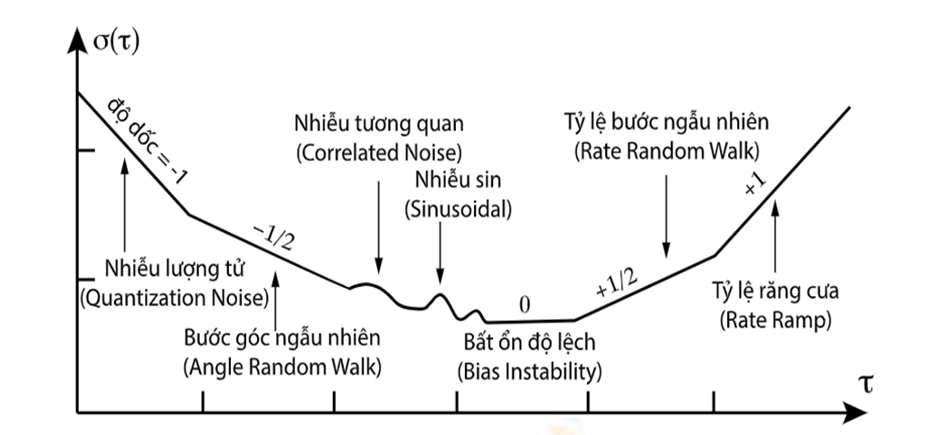
\includegraphics[width=1\textwidth]{images/allan.png}
		\caption{Minh hoạ kết quả phân tích đường cong Allan}
		\label{allan}
\end{figure}

\begin{figure}[!]
		\centering
 		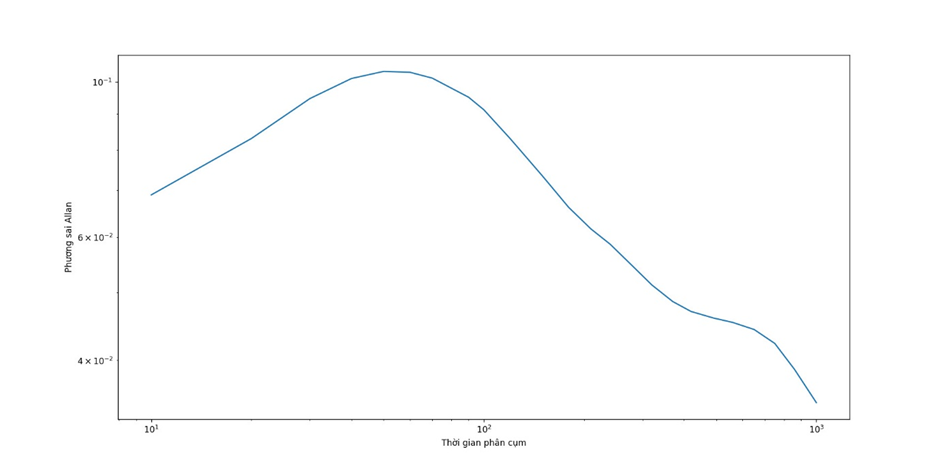
\includegraphics[width=1\textwidth]{images/allan_real.png}
		\caption{Biểu đồ phương sai Allan của trục x}
		\label{allan_real}
\end{figure}

Lỗi ngẫu nhiên phân tích theo phương sai Allan \cite{allan}. Phương sai Allan là phương pháp phân thích chuỗi dữ liệu trong miền thời gian để đo lường sự ổn định tần số trên miền tần số. Phương pháp này là một trong những phương pháp phổ biến nhất hiện nay để xác định và định lượng được nhiều loại nhiễu khác nhau tồn tại trong dữ liệu của cảm biến gia tốc, quán tính, cũng có thể sử dụng phương sai Allan để xác định các nhiễu nội tại trong một hệ thống như là một hàm trung bình cộng của thời gian. Các thành phần nhiễu cảm biến có thể xác định được bằng cách phân tích đồ thị log-log. Độ dốc đường cong Allan sẽ thể hiện các thành phần nhiễu khác nhau.

Tác giả thu tập được 1211210 mẫu dữ liệu khi để cảm biến đứng với tần số lấy mẫu là 10 Hz ở trong phòng với nhiệt độ bình thường. Kết quả đường cong Allan Hình \ref{allan_real} cho thấy nhiễu lượng tử xuất hiện chủ yếu là nhiễu lượng tử (Quantization noise) dựa trên việc đối chiếu hệ số góc với Hình \ref{allan_real}. Đây là nhưng nhiễu chủ yếu từ bản thân của cảm biến.


\begin{figure}[!]
		\centering
 		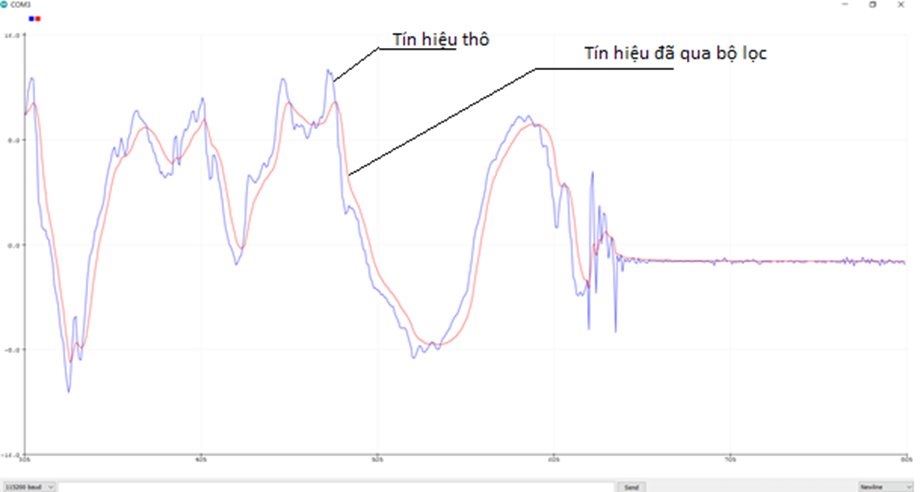
\includegraphics[width=1\textwidth]{images/kalman.png}
		\caption{Kết quả bộ lọc Kalman cho dữ liệu thô lấy trực tiếp từ trục X của cám biến gia tốc}
		\label{kalman}
\end{figure}
Trong khuôn khổ khoá luận, tác giả sử dụng bộ lọc Kalman để lọc các tín hiệu nhiễu đăc biệt là nhiễu lượng tử \cite{kalman}. Bộ lọc Kalman là thuật toán sử dụng chuỗi các giá trị đo lường, bị ảnh hưởng bởi nhiễu hoặc sai số, để ước đoán biến số nhằm tăng độ chính xác so với việc sử dụng duy nhất một giá trị đo lường. Bộ lọc Kalman là một bộ lọc đệ quy để ước lượng trạng thái của hệ thống tuyến tính, và cả hệ thống phi tuyến khi áp dụng phép ước lượng phi tuyến sang tuyến tính. Bộ lọc Kalman được ứng dụng rất nhiều trong lĩnh vực kĩ thuật, đặc biệt là lĩnh vực điều khiển. Tín hiệu sau khi được thu thâp sẽ được đi qua bộ lọc ở vi xử lý rồi mới được chuyển tới ứng dụng để hiển thị và lưu trữ. Bộ lọc đã được tác giả thực hiện lập trình và có kết quả như Hình ~\ref{kalman}. Kết quả cho thấy, bộ lọc Kalman đã lược bỏ dữ liệu ít ý nghĩa hoặc nhiễu (ồn) cho một đường biểu diễn mượt mà hơn.





\subsection{Xây dựng phần mềm ứng dụng}

Phần mềm ứng dụng được thiết kế với mục tiêu tạo thuận lợi cho người dung. Nhiệm vụ chính là thực hiện liên kết đến phần cứng và giao diện trực tiếp để người dùng thực hiện các thao tác. 

\begin{itemize}
    \item Ngôn ngữ: Dart
    
    \item Framework: Flutter
    
    \item Hệ điều hành: Android
    
    \item Kết nối với phần cứng: Ble
    
    \item Chức năng: Đảm bảo các yêu cầu cơ bản, thuận tiện cho người sử dụng.
\end{itemize}
\begin{figure}[!]
		\centering
 		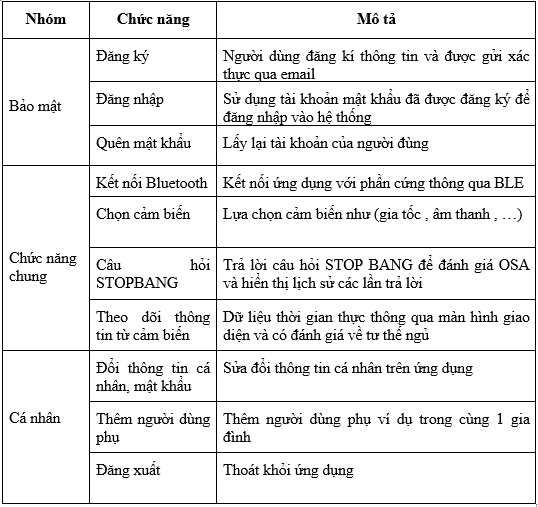
\includegraphics[width=1\textwidth]{images/app_flow.png}
		\caption{Các chức năng cơ bản của ứng dụng}
		\label{app_flow}
\end{figure}

Ứng dụng gồm 3 nhóm chức năng chính, Hình ~\ref{app_flow} bao gồm nhóm chức năng bảo mật, nhóm chức năng chung và nhóm chức năng cá nhân.
\begin{figure}[!]
		\centering
 		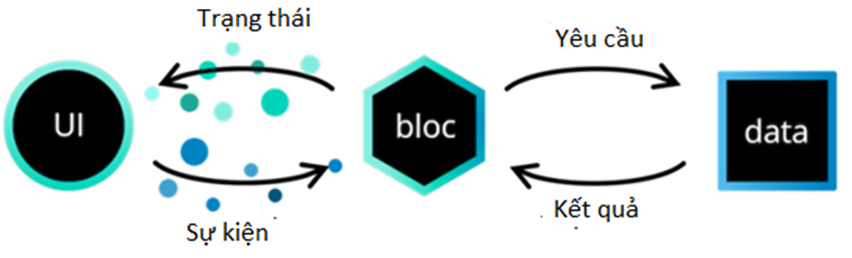
\includegraphics[width=0.8\textwidth]{images/flutter.png}
		\caption{Cấu trúc BLOC}
		\label{flutter}
\end{figure}


\begin{lstlisting}[float,language=dart,caption=Tập lệnh để tìm kiểm dịch vụ cảm biến ,label=flutterBle,captionpos=b]
StreamBuilder<List<BluetoothService>>(
      stream: device.services,
      initialData: [],
      builder: (c, snapshot) {
        if (snapshot.data!.length > 0) {
          isService = true;
        }
        BluetoothService serviceAcclerometer;
        if (snapshot.data == null || snapshot.data!.length == 0) {
          return Text("Please contact customer Service");
        }
        for (int i = 0; i < snapshot.data!.length; i++) {
          if (snapshot.data![i].uuid.toString() ==
              Constants.ACCLEROMETER_SERVICE) {
            accelerometerService = snapshot.data![i];
           }
        }
        if (accelerometerService == null) {
          return Text("Please contact customer Service");
        }
        for (int i = 0;
            i < accelerometerService!.characteristics.length;
            i++) {
          print(accelerometerService!.characteristics[i].uuid);
          if (accelerometerService!.characteristics[i].uuid
                  .toString() ==
              Constants.ACCLEROMETER_CHARACTION) {
            accelerometerCharactis =
                accelerometerService!.characteristics[i];
          }
        }
}));

\end{lstlisting}

\begin{lstlisting}[float,language=Java,caption=Tập lệnh đọc dữ liệu từ BLE, label=flutter_get_data,captionpos=b]
void setupPosition(void)
{
 
  positionService.begin();

  accelerometerCharacter.setProperties(CHR_PROPS_NOTIFY+CHR_PROPS_READ+CHR_PROPS_WRITE );
  accelerometerCharacter.setPermission(SECMODE_OPEN, SECMODE_NO_ACCESS);
  accelerometerCharacter.setFixedLen(9);
  accelerometerCharacter.setCccdWriteCallback(cccd_callback);  // Optionally capture CCCD updates
  accelerometerCharacter.begin();
  uint8_t accelerometerData[9] = { 0b00000000, 0b00000000, 0b00000000,0b00000000,0b00000000,0b00000000,0b00000000,0b00000000,0b00000000}; // Set the characteristic to use 8-bit values, with the sensor connected and detected
  accelerometerCharacter.write(accelerometerData, 9);

  gyroscopeCharacter.setProperties(CHR_PROPS_READ);
  gyroscopeCharacter.setPermission(SECMODE_OPEN, SECMODE_NO_ACCESS);
  gyroscopeCharacter.setFixedLen(1);
  gyroscopeCharacter.begin();
  gyroscopeCharacter.write8(2);    // Set the characteristic to 'Wrist' (2)
}

\end{lstlisting}



\textbf{Flutter} là cross-platform dành cho ứng dụng di động viết theo kiểu hướng đối tượng. Nó có thể lập trình cho cả ứng dụng trên nền tảng Android và IOS. Khả năng phát triển nhanh chóng có nhiều thành phần (Widget) có sẵn, đẹp, dễ sử dụng và có nhiều thư viện và cộng đồng sử dụng. Trong ứng dụng này tác giả sử dụng Bloc là một thư viện để quản lý trạng thái cho ứng dụng Flutter B.L.o.C (Business Logic Component). Nhận sự kiện như là đầu vào và trả về kết quả là trạng thái. Bloc được xây dựng dựa trên RxDart. Chúng ta có thể chia kiến trúc Flutter thành 3 lớp như Hình ~\ref{flutter}. Trong đó UI là giao diện của người dùng, nơi người dùng nhìn thấy dữ liệu, thao tác. Bloc là thư viện để quản lý các trạng thái của ứng dụng. Các sự kiện là các hành động như ấn nút, nhập dữ liệu, v.v.




Khi đã lấy được đối tượng tính năng (charactis instance), tác giả sẽ liên tục đẩy  hành động đọc (read) từ phần mềm ứng dụng đến vi điều khiển. Khi vi điều khiển nhận được hành động đọc được gửi từ ứng dụng sẽ trả lại tín hiệu của cảm biến. Ở đây, các BLE gửi các dữ liệu theo định dạng là mảng các phần tử có kiểu là UInt8. Do đó, sau khi nhận được dữ liệu từ phần cứng, dữ liệu dạng UInt8 được chuyển về dạng Number. Với quy trình như vậy, hệ thống có độ trễ rất thấp (real time). Cuối cùng việc lưu trữ thông tin cảm biến được thông qua giao thức Giao thức Truyền tải Siêu Văn Bản (Hyper Text Transfer Protocol - HTTP) truyền lên phía máy chủ(backend) và được thực hiện ở đoạn Mã \ref{flutter_get_data}.
\begin{lstlisting}[float,language=C,caption="Cấu trúc dữ liệu của phần nội dung đẩy lên máy chủ",label=format_ble,captionpos=b]
{
    "value": "0.88%0.66%0.99@2022-01-01/0.88%0.66%0.99@2022-01-01/0.88%0.66%0.99@2022-01-01",
    "customer": "62a5f5672ad9c724ef117d76"
}

\end{lstlisting}

Việc đẩy tín hiệu như vậy, tránh được tình trạng tắc nghẽn ở phía backend. Trong thời gian tới, cơ chế nghe/nhận (pub/sub) sẽ được áp dụng để tránh tình trạng gọi các yêu cầu (request) liên tục. Dữ liệu sẽ được đẩy lên theo định dạng Mã \ref{format_ble}:

Ngoài ra, tác giả phát triển thêm tính năng bộ câu hỏi STOPBANG nhằm đánh giá ban đầu người dùng. Và những dữ liệu này có trọng số quan trọng trong việc đánh giá chỉ số AHI sử dụng học máy sau này. Tính năng thêm người dùng được sử dụng để tránh phải thao tác tạo mới nhiều lần nhưng vẫn giữ được tính bảo mật, lấy lại dữ liệu khi mà quên tài khoản, mật khẩu.



\subsection{Thiết kế và xây dựng hệ thống lưu trữ   }
\begin{figure}[b!]
		\centering
 		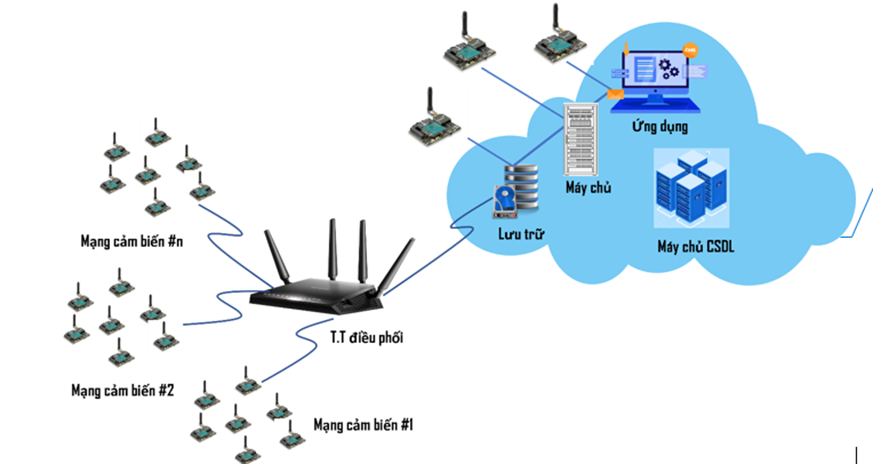
\includegraphics[width=0.8\textwidth]{images/cloud.png}
		\caption{Mô hình tích hợp giữa mạng cảm biến và cấu trúc dữ liệu đám mây}
		\label{cloud}
\end{figure}


Dữ liệu (data) là cơ sở của công nghệ trí tuệ nhân tạo để phân tích, đánh giá, dự đoán nhiều lĩnh vực trong cuộc sống. Vì mỗi thiết bị phần cứng chỉ có không gian bộ nhớ có hạn nên việc lưu trữ trên hệ thống đám mây (cloud) đang là phương pháp phổ biến nhất Hình ~\ref{cloud}. Việc triển khai dữ liệu lên cloud giúp xóa bỏ khoảng cách địa lý, thuận tiện cho việc trích xuất bất kì nơi nào miễn là có kết nối internet, qua đó có thể dễ dàng xuất ra các file text, csv và thuận tiện chia sẻ trao đổi với các nhóm nghiên cứu khác. Mục tiêu dài hạn của hướng nghiên cứu này là việc sử dụng cơ sở dữ liệu đủ lớn cho các mô hình toán học nhằm dự đoán, hỗ trợ ra quyết định trong các hoạt động sàng lọc và chẩn đoán chứng \gls{OSA} ở người. 


\begin{itemize}
    \item MongoDB được thiết kế để có thể truy vấn hiệu quả các bộ dữ liệu rất lớn, ngay cả khi dữ liệu được phân chia trên nhiều máy chủ, miễn là có thể chọn share key đoạn phù hợp khớp với các truy vấn đọc phổ biến nhất của mình.
    
    \item Hỗ trợ tốt đối với dữ liệu TimeStamp.
    
    \item Các chỉ mục được phân nhóm tối ưu hóa hiệu suất và lưu trữ chỉ mục.
    
    \item Tự động xóa dữ liệu cũ hơn. Lưu trữ dữ liệu bằng kho lưu trữ trực tuyến Atlas và dễ mở rộng
\end{itemize}


\begin{figure}[!]
		\centering
 		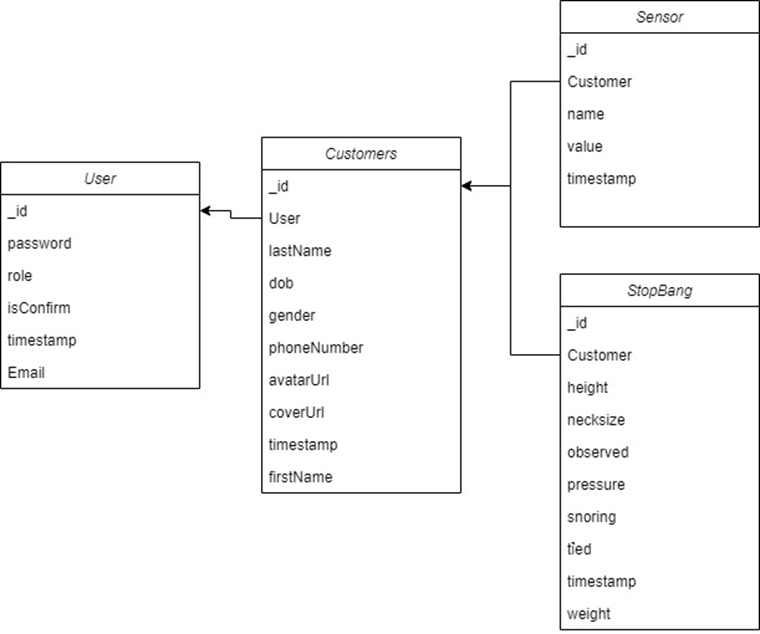
\includegraphics[width=1\textwidth]{images/csdl.png}
		\caption{Cấu trúc lưu trữ dữ liệu}
		\label{cloud}
\end{figure}
\begin{figure}[b!]
		\centering
 		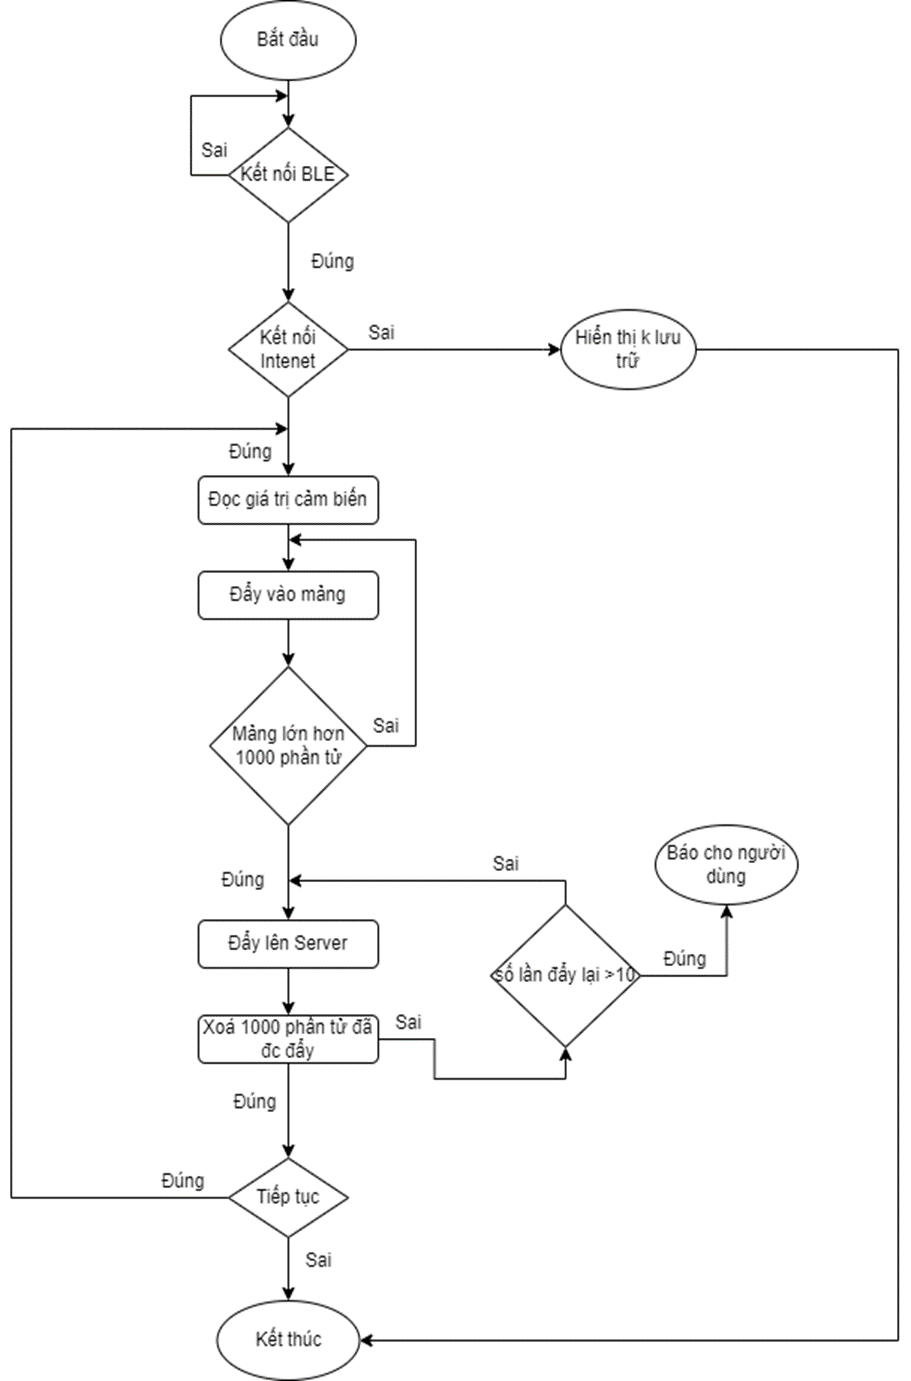
\includegraphics[width=0.9\textwidth]{images/flow_http.png}
		\caption{Lưu đồ thuật toán lưu trữ dữ liệu cảm biến}
		\label{flow_http}
\end{figure}


Trong khóa luận này, phần máy chủ của hệ thống được xây dựng trên nền tảng NodeJs và triển khai trên AWS - nền tảng đám mây cho phép các lập trình viên xây dựng, triển khai, quản lý và mở rộng ứng dụng. Cơ sở dữ liệu sử dụng trên nền tảng MongoDb Atlas hỗ trợ free 500Mb.

Để tránh tình trạng quá tải server khi có quá nhiều yêu cầu truy cập cùng lúc đến, tác giả đã gộp các giá trị cảm biến vào 1 mảng 1000 phần tử rồi đẩy mảng đó lên backend. Việc lưu trữ này yêu cầu phải xác định được chính xác thời gian của từng giá trị của biến số trên ứng dụng di động và truyền lên cùng giá trị của 3 trục x, y, z. Việc lưu trữ dữ liệu được tác giả mô tả như lược đồ, Hình ~\ref{flow_http} bao gồm 2 trường hợp:



\begin{itemize}
    \item Khi người dùng không có kết nối mạng thì người dùng chỉ được phép truy cập vào BLE và hiển thị dữ liệu không có lưu trữ.
    
    \item Khi trường hợp người dùng đã đăng nhập và có kết nối mạng thì ứng dụng sẽ tự động lưu trữ khi thu thập đủ 1000 giá trị. Nếu không thành công 10 lần sẽ báo cho người dùng.
\end{itemize}


\subsection{Tìm hiểu, ứng dụng phân loại tư thế ngủ bằng học máy  }

Tác giả cũng đã tìm hiểu nhiều mô hình, phương pháp để phân loại các tư thế ngủ, tư thế cơ bản của con người và đánh giá chỉ số AHI dự trên các tín hiệu cảm biến thu được. Các bước cơ bản để tiến hành dự án học máy liên quan đến các tín hiệu cảm biến:


\begin{figure}[b!]
		\centering
 		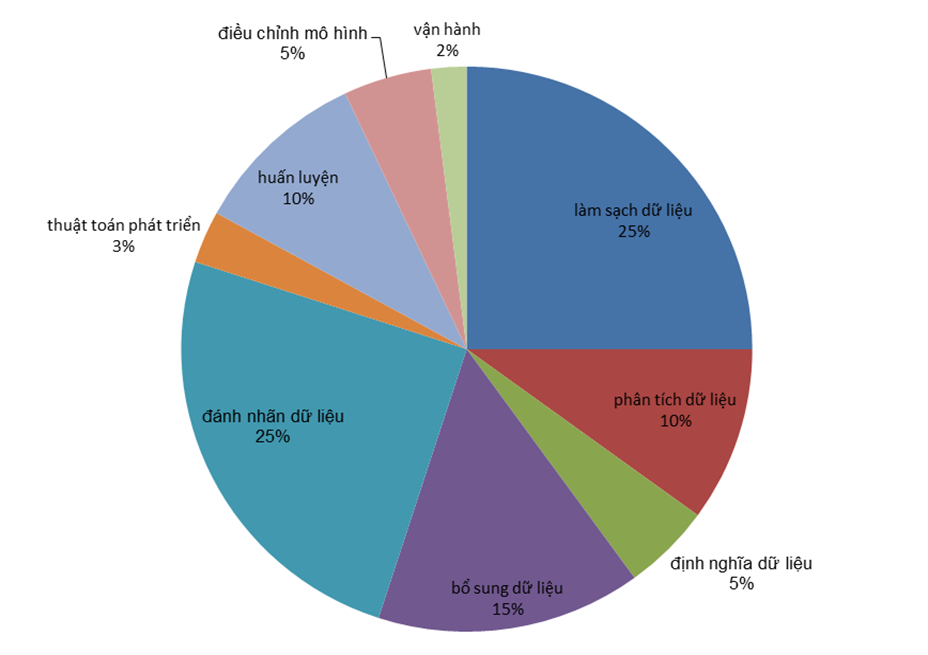
\includegraphics[width=1\textwidth]{images/hocmay_time.png}
		\caption{Phân bố thời gian sử dụng đối với dự án học máy}
		\label{hocmay_time}
\end{figure}

\begin{itemize}
    \item Thu thập dự liệu (bao gồm thu thập và gắn nhãn cho dữ liệu)
    
    \item Khám phá dữ liệu (đánh giá cân bằng dữ liệu, tỉ lệ dữ liệu có ý nghĩa)
    
    \item Chuẩn bị dữ liệu (làm sạch dữ liệu, tạo ra các đặc tính trên miền thời gian và miền tần số)
    
    \item Mô hình hoá dữ liệu (lựa chọn ra các mô hình phù hợp)
    
    \item Lựa chọn tính năng (lựa chọn ra các tính năng có ý nghĩa cao đối với mô hình)

    \item Tinh chỉnh mô hình
\end{itemize}

Jeng PY và cộng sự đã đề xuất chế tạo 2 thiết bị đeo ở cổ và ở cổ tay để đánh giá tư thế ngủ ở người \cite{Jeng}. Trong dự án này, tín hiệu thu được ở thiết bị đeo ở tay được chia thành những cửa sổ 1 giây rồi trích xuất các tính năng trên cửa sổ đó. Cảm biến đeo ở cổ sẽ được sử dụng để lấy nhãn tín hiệu theo phương pháp lấy đa số của tín hiệu trong cửa sổ. Nhóm tác giả đã sử dụng mô hình SVM và RF để đánh giá và đạt được kết quả có độ chính xác lần lượt là 82\% và 72\%. Nhóm của Saha S., Kabir M và cộng sự đã tiến hành nghiên cứu 1 thiết bị đeo được sử dụng bao gồm cảm biến gia tốc, cảm biến âm trên 31 đối tượng thử nghiệm. Sau đó họ tiến hành loại bỏ các bộ dữ liệu có độ dài dưới 2 giờ và cuối cùng sử dụng so sánh ngưỡng để xác định chứng OSA bằng việc phân chia các cửa sổ 10s với độ lặp 80\% \cite{Saha}. Trong khi đó, nhóm của Syeda Zuriat-e-Zehra Ali và cộng sử đã nghiên cứu và thử nghiệm thiết bị gối ngủ để tự điều chỉnh hoặc báo hiệu khi có chứng ngưng thở khi ngủ dựa trên các tín hiệu thô như nồng độ Oxi trong máu, nhịp tim [27]. Jarvis L, Moninger S và cộng sử đã trình bày hệ thống phát hiện đánh giá 5 tư thế gồm nằm, nằm tựa, ngồi thẳng, đứng, đi bộ với tập dữ liệu đươc lấy từ 2 cảm biến gắn ở cổ và đùi \cite{Syeda}. Dữ liệu được lấy mẫu với tần số 25 Hz sau đó được lưu vào bộ nhớ cục bộ trên điện thoại rồi gửi bản csv qua mail. Mô hình học máy gồm hồi quy logistic, SVM, DT với độ chính xác cao > 96\% đã được sử dụng đánh giá tập dữ liệu gồm 6 hành động thường ngày của con người như đứng, ngồi, đi bộ, lên cầu thang, xuống cầu thang và nằm \cite{Uday}. Nhóm nghiên cứu của Gomes E, Bertini L và cộng sự đã nghiên cứu, xây dựng, đánh giá giữa 3 mô hình: K-Nearest-Neighbor (KNN), cây quyết định (Decision tree) và SVM. Trong các bước tiền xử lý các tác giả đã phân đoạn dữ liệu theo cửa sổ 2.5s không che phủ sau đó phân tích, chuẩn hoá dữ liệu và đã có độ chính xác > 97\% đối với việc phát hiện tư thế. Ở Việt Nam, nhóm tác gủa Vũ Ngọc Thanh Sang và Nguyễn Đức Thắng đã phát triển thiết bị thu thâp dữ liệu từ điện thoại sau đó qua các bước xử lý dữ liệu, trích xuất tính năng và phân loại bằng các mô hình K-hàng xóm gần nhất (KNN) với độ chính xác là 100\% với toàn bộ tư thế ngoại trừ lái xe là 80\% \cite{Sang}. Qua tổng quan tài liệu tác giả nhận thấy các phương pháp học máy cổ điển đang chiến ưu thế hơn so với các phương pháp học sâu vì phát triển nhanh và dễ dàng và phù hợp với tính chất của bài toán đánh giá các tư thế của con người sử dụng cảm biến gia tốc. Trong đó, nổi bật lên là mô hình SVM, hồi quy Logistic và Random Forest. Từ đó, tác giả sẽ tập trung tìm hiểu và hướng tới áp dụng cho tập dữ liệu của tác giả.


\textbf{Hồi quy logistic - LR}: Đây là phương thức tốt nhất cho các vấn đề phân loại nhị phân (vấn đề với hai lớp giá trị). Hồi quy logistic giống như hồi quy tuyến tính với mục đích là để tìm ra các giá trị cho các hệ số mà trọng lượng mỗi biến đầu vào. Không giống như hồi quy tuyến tính, dự đoán đầu ra được chuyển đổi bằng cách sử dụng một hàm không tuyến tính được gọi là hàm logistic. Hàm logistic trông giống như một chữ S lớn và sẽ biến đổi bất kỳ giá trị nào thành 0-1. Tuy nhiên, nhược điểm của nó là chỉ giải quyết được bài toán phân loại 2 lớp. Để giải quyết được những bài toán đa lớp chúng ta có thể sử dụng mô hình Softmax Logistic là dạng tổng quát của hồi quy Logistic.

\textbf{Máy vec tơ hỗ trợ (Support vector machines - SVM)}: xây dựng một mặt siêu phẳng được sử dụng để phân chia không gian biến đầu vào. Trong SVM, một mặt siêu phẳng được chọn để phân tách tốt nhất các điểm trong không gian các biến đầu vào theo lớp của chúng, hoặc là lớp 0 hoặc lớp 1. Trong không gian hai chiều, có thể hình dung nó như một đường thẳng và giả sử rằng tất cả các biến đầu vào có thể được tách hoàn toàn bằng đường thẳng này. Thuật toán SVM tìm ra các hệ số dẫn đến sự phân tách tốt nhất của các lớp theo mặt siêu phẳng Hình ~\ref{svm}.


\begin{figure}
    \centering
    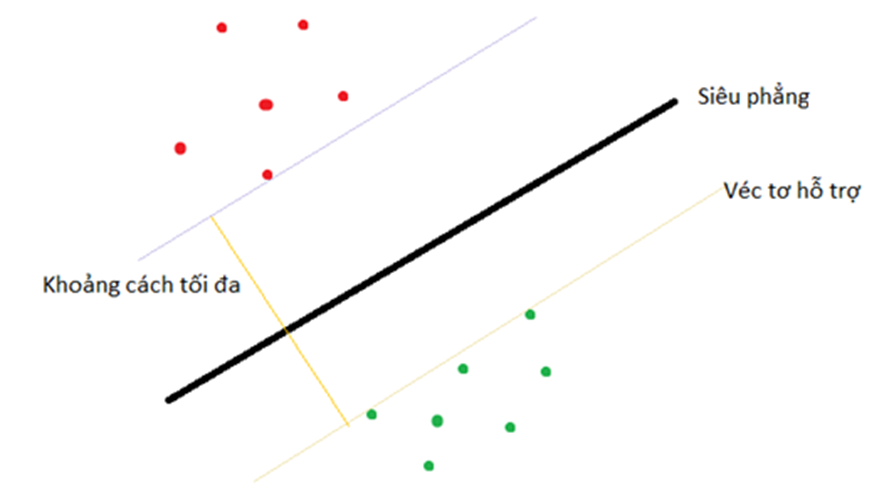
\includegraphics[width=1\linewidth]{images/svm.png}
    \caption{Tối ưu siêu phẳng sử dụng thuật toán SVM}
    \label{svm}
\end{figure}
Khoảng cách giữa mặt siêu phẳng và điểm dữ liệu gần nhất được gọi là biên. Mặt siêu phẳng tốt nhất hoặc tối ưu có thể tách riêng hai lớp là dòng có biên lớn nhất. Chỉ những điểm này có liên quan đến việc xác định hyperplane và trong việc xây dựng các điểm phân loại. Những điểm này được gọi là các vector hỗ trợ. Chúng hỗ trợ hoặc xác định hyperplane. Trong thực tế, một thuật toán tối ưu được sử dụng để tìm các giá trị cho các hệ số tối đa hóa biên. SVM có thể là một trong những phương pháp phân loại hàng đầu mạnh mẽ nhất và đáng thử trên tập dữ liệu. Cũng như hồi quy Logistic thì SVM cũng chỉ sử dụng để phân loại nhị phân. Để giải quyết vấn đề này thì có 2 phương pháp:

\begin{figure}
    \centering
    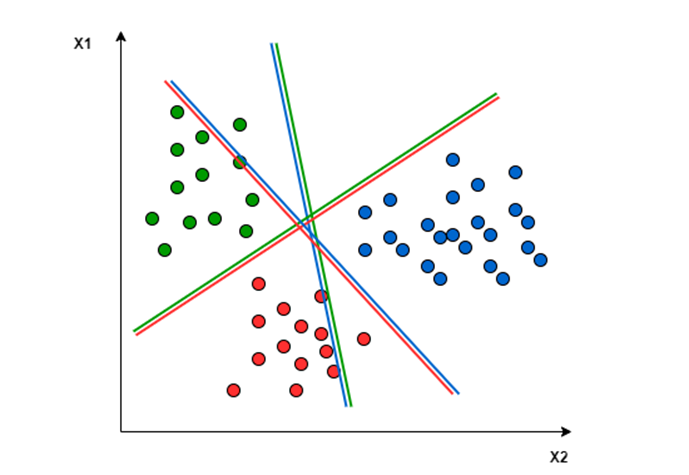
\includegraphics[width=0.6\linewidth]{images/svm_ovso.png}
    \caption{Thuật toán một với một}
    \label{svm_ovso}
\end{figure}



\begin{figure}
    \centering
    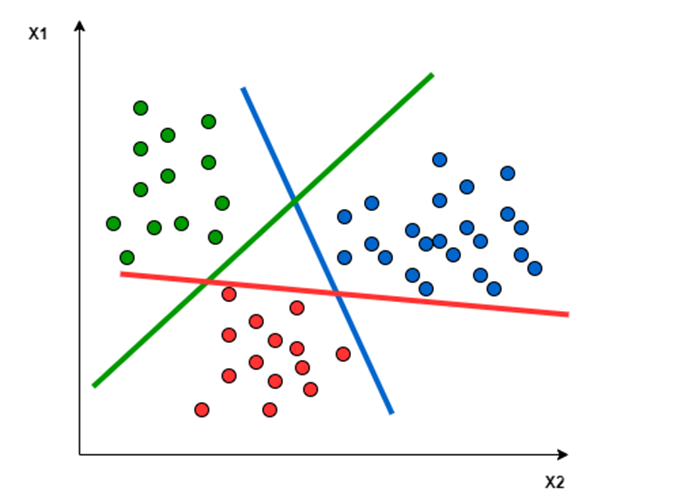
\includegraphics[width=0.6\linewidth]{images/ovsr.png}
    \caption{Thuật toán một với nhiều}
    \label{ovsr}
\end{figure}

\begin{itemize}
    \item Một với một (one vs one): Một mặt siêu phẳng được thiết lập để phân tách giữa hai lớp, bỏ qua các điểm của lớp thứ ba. Điều này có nghĩa là sự phân tách chỉ tính đến điểm của hai lớp trong sự phân tách hiện tại. Ví dụ: đường màu đỏ-xanh dương sẽ tách tối đa khoảng cách chỉ giữa các điểm màu xanh lam và màu đỏ Hình ~\ref{svm_ovso}.
    
    \item Một với nhiều (one vs rest): Cần một mặt siêu phẳng để tách biệt giữa một lớp và tất cả các lớp khác cùng một lúc. Điều này có nghĩa là sự tách biệt có tính đến tất cả các điểm, chia chúng thành hai nhóm; một nhóm cho các điểm của lớp và một nhóm cho tất cả các điểm khác. Ví dụ: đường màu sẽ tách tối đa hóa khoảng cách giữa các điểm màu lục và tất cả các điểm khác cùng một lúc Hình ~\ref{ovsr}.
\end{itemize}






\textbf{Rừng ngẫu nhiên (Random Forest - RF)}: được xây dựng trên cơ sở thuật toán Decision Tree (cây quyết định). Mỗi cây quyết định sẽ khác nhau (có yếu tố ngẫu nhiên khác nhau). Sau đó kết quả dự đoán được tổng hợp từ các cây quyết định. Trong thuật toán Decision Tree, khi xây dựng cây quyết định nếu để độ sâu tùy ý thì cây sẽ phân loại đúng hết các dữ liệu trong tập training dẫn đến mô hình có thể dự đoán tệ trên tập validation/test, khi đó mô hình bị quá khớp (overfitting).
Thuật toán Random Forest gồm nhiều cây quyết định, mỗi cây quyết định đều có những yếu tố ngẫu nhiên:
Lấy ngẫu nhiên dữ liệu để xây dựng cây quyết định.
Lấy ngẫu nhiên các thuộc tính để xây dựng cây quyết định.
Do mỗi cây quyết định trong thuật toán Random Forest không dùng tất cả dữ liệu training, cũng như không dùng tất cả các thuộc tính của dữ liệu để xây dựng cây nên mỗi cây có thể sẽ dự đoán không tốt, khi đó mỗi mô hình cây quyết định không bị overfitting mà có thế bị underfitting, hay nói cách khác là mô hình có high bias. Tuy nhiên, kết quả cuối cùng của thuật toán Random Forest lại tổng hợp từ nhiều cây quyết định, thế nên thông tin từ các cây sẽ bổ sung thông tin cho nhau, dẫn đến mô hình có low bias và low variance, hay mô hình có kết quả dự đoán tốt.
	Những kiến thức cơ bản về học máy sẽ được ứng dụng sâu trong những nghiên cứu tới đây của tác giả.

